\section{Conclusiones}



\subsection{Resumen de la investigación}

\begin{frame}
    \frametitle{OCS-WAF}

    \begin{itemize}
        \item
        Implementación de un WAF para protección de múltiples aplicaciones
        web

        \item
        Detección de anomalías en mensajes HTTP mediante clasificadores
        One-Class SVM
    \end{itemize}

    \begin{center}
        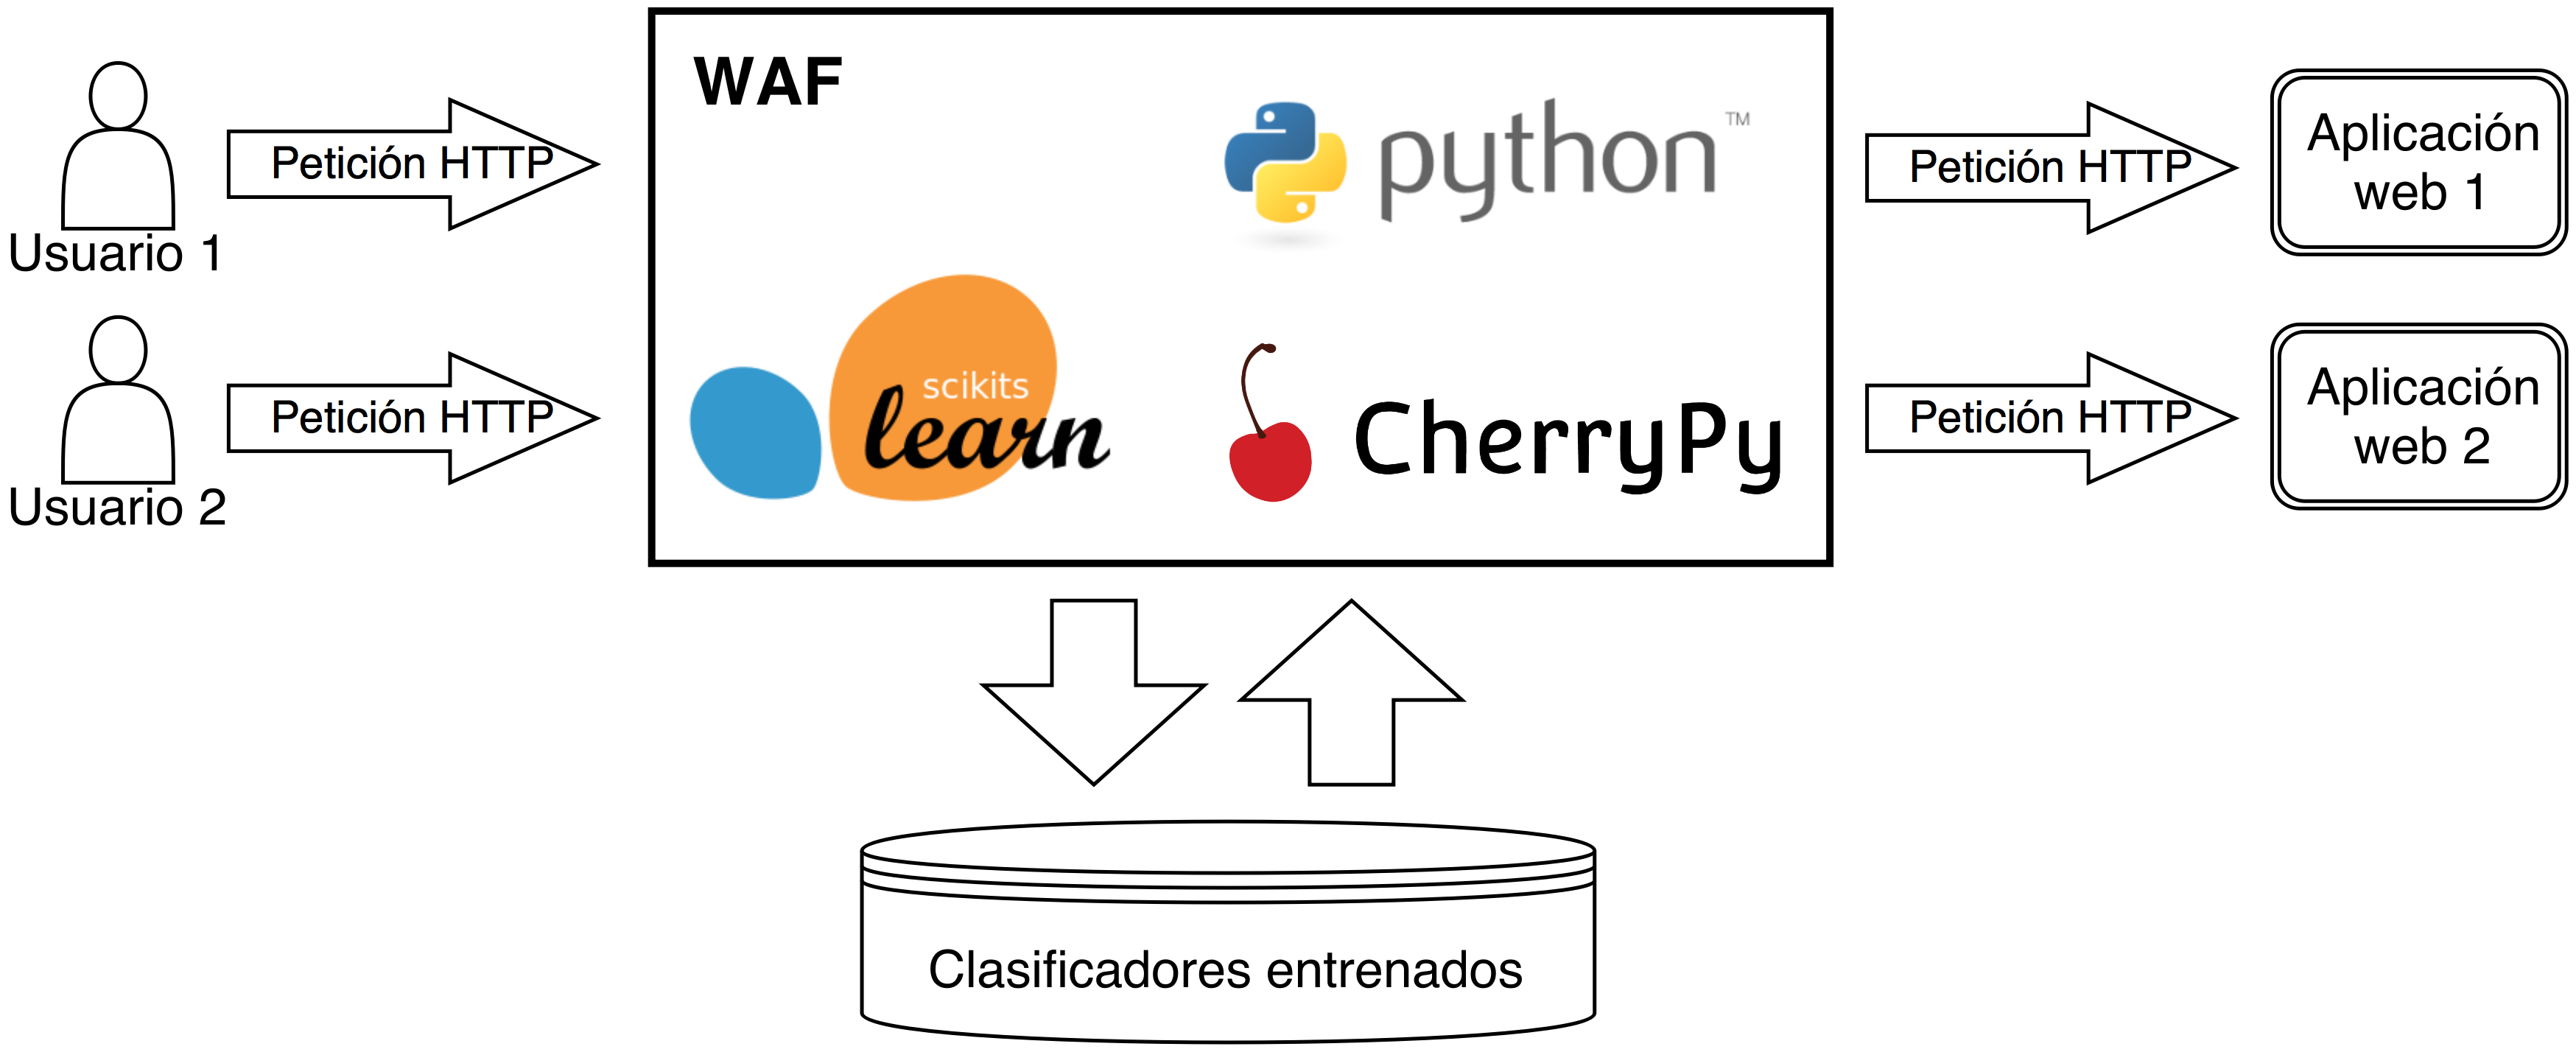
\includegraphics[width=\textwidth]{images/waf-diagram-overview.png}
    \end{center}
\end{frame}



\subsection{Logro de los objetivos}

\begin{frame}
    \frametitle{Objetivos específicos}

    \begin{enumerate}[<+(1)->]
        \item
        Diseñar procesos de extracción de características (\textit{features})
        específicamente para mensajes HTTP, basado en aportes de otros
        investigadores de la literatura.

        \begin{itemize}[<.->]
            \item
            Diseño de nuevos procesos de extracción de \textit{features}
            para mensajes HTTP
        \end{itemize}

        \item
        Implementar un WAF basado en anomalías, utilizando los procesos de
        extracción de \textit{features} diseñados junto con clasificadores
        One-Class SVM.

        \begin{itemize}[<.->]
            \item
            Implementación de OCS-WAF
        \end{itemize}

        \savemynewenumi
    \end{enumerate}
\end{frame}

\begin{frame}
    \frametitle{Objetivos específicos}

    \begin{enumerate}[<+->]
        \contmynewenumi

        \item
        Evaluar la eficacia del WAF implementado en cuanto a la detección
        de mensajes HTTP anómalos.

        \begin{itemize}[<.->]
            \item
            Pruebas de eficacia de detección con un
            TPR de \num{0.93},
            FPR de \num{0.03} y
            F$_{1}$-\textit{score} de \num{0.95}
        \end{itemize}

        \item
        Analizar la viabilidad de utilizar el WAF implementado para
        detección de ataques en tiempo real.

        \begin{itemize}[<.->]
            \item
            Realización de pruebas de impacto de OCS-WAF sobre el tiempo
            de respuesta de las aplicaciones protegidas
        \end{itemize}
    \end{enumerate}
\end{frame}

\begin{frame}
    \frametitle{Objetivo general}

    \begin{itemize}[<+(1)->]
        \item
        Detectar mensajes HTTP anómalos entre las aplicaciones web y
        sus usuarios con el fin de mitigar los riesgos de ataques contra
        dichas aplicaciones, utilizando un WAF basado en clasificadores
        One-Class SVM.

        \begin{itemize}[<.->]
            \item
            Detección de mensajes HTTP anómalos con OCS-WAF
        \end{itemize}
    \end{itemize}
\end{frame}



\subsection{Trabajos futuros}

\begin{frame}
    \frametitle{Ideas para trabajos futuros}

    \begin{itemize}[<+(1)->]
        \item
        Realizar pruebas con otros conjuntos de datos.

        \item
        Explorar otras características de los mensajes HTTP.

        \item
        Extender para incluir cuerpos de otros formatos, por ejemplo
        datos binario, JSON, XML, entre otros.

        \item
        Extender para incluir mensajes HTTP/2.

        \item
        Explorar la posibilidad de paralelizar el proceso de entrenamiento
        en OCS-WAF.
    \end{itemize}
\end{frame}



\subsection{Publicaciones}

\begin{frame}
    \frametitle{Publicación de nuestro trabajo}

    \begin{itemize}
        \footnotesize

        \item
        \textbf{Título:}
        Anomaly-based Web Application Firewall using HTTP-specific features
        and One-Class SVM
    \end{itemize}

    \begin{block}{\small WRSeg 2017}
        \begin{columns}
            \column{0.6\textwidth}
            \begin{itemize}
                \footnotesize

                \item
                Workshop Regional de Segurança da Informação e
                Sistemas Computacionais

                \item
                Santa María, Brasil

                \item
                25 de Setiembre 2017
            \end{itemize}

            \column{0.4\textwidth}
            \begin{center}
                
\includegraphics[width=\textwidth]{images/logo-errc2017.png}
            \end{center}
        \end{columns}
    \end{block}

    \begin{block}{\small Revista REABTIC}
        \begin{columns}
            \column{0.6\textwidth}
            \begin{itemize}
                \footnotesize

                \item
                Revista Eletrônica Argentina-Brasil de Tecnologias da Informação
                e da Comunicação

                \item
                Enviado para revisión
            \end{itemize}

            \column{0.4\textwidth}
            \begin{center}
                
\includegraphics[width=\textwidth]{images/logo-reabtic.png}
            \end{center}
        \end{columns}
    \end{block}
\end{frame}
